\chapter{Get Serious}

These notes follow a Jim Rohn lecture from a curated LazyingArt LLC playlist rather than from a classroom course with surviving board work. No validated frame-backed equations or diagrams remain for this talk, so the formal notation below is transcript-derived and, where necessary, cautiously cleaned up. The lecture's mathematics is therefore programmatic rather than algebraic: numbered imperatives, target arithmetic, state-like seasons, and compact rules for discipline, neglect, and response. Its formal spine may be written at once as
\begin{equation}
G_6 := (\text{get serious},\ \text{get smart},\ \text{get going},\ \text{get better},\ \text{get excited},\ \text{get away}).
\end{equation}
What matters is not merely the list, but the order. Each step is introduced because the previous one is insufficient by itself.

\section{Get Serious: Life, Stakes, and the \$400$ Million Goal}

The lecture opens with pressure, not with explanation. We are first told to get serious, and only then are we shown why. Life, in Rohn's first compact formulation, is not a neutral condition but a continual resistance:
\begin{equation}
\text{life} := \text{the struggle to keep death at a respectable distance}.
\end{equation}
This is the opening axiom of tone. It tells us why the speaker refuses a merely entertaining meeting. If life, health, family support, and the future are serious, then the room must be serious too.

From there the lecture broadens the frame. The same world contains both visible triumph and visible collapse:
\begin{equation}
\text{same historical moment} = \text{best of times for some} + \text{worst of times for others}.
\end{equation}
This equation is editorial, but the contrast is exactly the lecture's own. Some are taking home diamonds and million-dollar incomes; others, in the same historical moment, are still living in what he calls the worst of times. That widening matters. It prevents seriousness from collapsing into private mood. We are already being asked to see a divided world.

Only after this does Rohn give seriousness a measurable object. The meeting is not to stay in the register of tone alone. It is supposed to take hold of a target, and the target is the \$400 million goal. He works it out by deliberately simple division:
\begin{align}
\$400\,\text{million}/400 &= \$1\,\text{million},\\
\$400\,\text{million}/800 &= \$0.5\,\text{million}.
\end{align}
The arithmetic is elementary on purpose. A large collective ambition is brought down to a share that can be mentally owned. At the same time the lecture refuses to let the number remain only a number. The figure stands for healing, restoration, encouragement, and touched lives. Seriousness becomes measurable, but it does not become merely financial.

\subsection{Question \& Answer}

Question: If life is serious for everyone, why do outcomes diverge so much?

Answer: The lecture first raises this question before it fully answers it. At this stage the answer is only partial: the seriousness of life is universal, but response is not. The same historical moment contains best times and worst times because shared conditions do not by themselves determine destination. The full explanation will come through learning, philosophy, and execution; but the question must be felt here, at the opening, or the rest of the program loses its necessity.

\section{Get Smart: Education Before Motivation}

Once seriousness has been established and given a target, the lecture turns sharply against a familiar mistake. We might think that after naming the goal all we need is more excitement. Rohn rejects that at once. The beginning of change is education. He even gives the point a practical rhythm: one way to learn to do it right is to do it wrong, provided one does not take too long learning the lesson. A call goes badly; the answer is not despair but another call.

The lecture's governing claims here are direct:
\begin{align}
\text{learning} &\Rightarrow \text{wealth},\\
\text{learning} &\Rightarrow \text{life change}.
\end{align}
We are told not to be lazy in learning, not to be lazy in picking up ideas, and not to be lazy in learning from our own experience. The testimonials from the stage are therefore not decoration. They are part of the educational method.

Against this the lecture places a deliberately rough negative correction:
\begin{equation}
\text{motivation alone} \not\Rightarrow \text{reliable results}.
\end{equation}
The point is not that motivation has no place. The point is that motivation without sense merely intensifies what is already there. The lecture's preferred form of motivation is the proof of success, the visible work of hands, the example of people who have done the job. That is why repetition matters so much here. Having heard a class once is no sign one has got it. Listening once to a tape is no sign one has absorbed it. The speech insists on hearing again, reviewing again, and learning again.

\subsection{Question \& Answer}

Question: Why is motivation not enough?

Answer: Because the lecture treats motivation as an amplifier rather than as a foundation. If understanding is weak, motivation only gives us a louder version of the same weakness. Education, by contrast, changes what we can see and therefore what we can do. The order is not
\begin{equation}
\text{goal} \to \text{excitement} \to \text{automatic success},
\end{equation}
but rather
\begin{equation}
\text{goal} \to \text{learning} \to \text{better action}.
\end{equation}

\section{Philosophy as the Set of the Sail}

The lecture now asks the deeper question that has been waiting since the beginning: what actually makes outcomes diverge under common conditions? Rohn's answer is philosophy, and he gives it in the cleanest conceptual model of the talk. Each person's philosophy is like the set of the sail. The same wind blows on all of us:
\begin{equation}
\text{same wind} \neq \text{same destination}.
\end{equation}
This is the decisive step. Conditions are shared; results are not. Therefore the explanation cannot stop with the wind. In cautious editorial shorthand we may write
\begin{equation}
\text{destination} \approx \text{common wind} + \text{personal sail-setting}.
\end{equation}
The approximation sign matters. This is not a literal board equation from the room; it is a faithful compression of the spoken model.

Rohn immediately uses the analogy to close down several evasions. We are not to ask for a more favorable wind. We are not to curse the economy, the government, the marketplace, or the fact that this is the only planet we have. We are to set a better sail. The lecture phrases the correction as paired wishes:
\begin{align}
\text{Don't wish it were easier};\qquad &\text{wish you were better},\\
\text{Don't wish for fewer problems};\qquad &\text{wish for more skills}.
\end{align}
This is the moment when the talk becomes fully pedagogical. Learning is not simply the accumulation of ideas. It is the formation of a philosophy that can direct a life under unchanged conditions.

The business setting is preserved here as well. We are told that Herbalife's philosophy has carried it to extraordinary heights, and the example given is practical rather than mystical: those who do the work get the pay. The point is not that philosophy floats above execution, but that it governs it.

\subsection{Question \& Answer}

Question: If the same wind blows on us all, what actually changes the destination?

Answer: In the lecture's own structure, it is not the wind but the sail-setting. Shared conditions give us the field within which we move; personal philosophy gives us orientation within that field. That is why the next step must be action. If philosophy never reaches conduct, it remains only spoken admiration for a better sail.

\section{Get Going: Neglect, Small Disciplines, and the Wrong Track}

The lecture's next move is almost algorithmic. Ideas are compared to seeds, and the point is obvious once said aloud: seeds admired are not seeds planted. Intelligence without execution does not yet produce a future. We are therefore told to get going.

Rohn's spoken pattern is repetitive because the logic depends on repetition. It can be written first in the more literal examples:
\begin{align}
\text{should walk} + \text{don't walk} &\Rightarrow \text{wrong track},\\
\text{should read} + \text{don't read} &\Rightarrow \text{wrong track},\\
\text{should call} + \text{don't call} &\Rightarrow \text{wrong track},\\
\text{should change} + \text{don't change} &\Rightarrow \text{wrong track}.
\end{align}
Then the lecture's pattern can be compressed, cautiously, into
\begin{equation}
\text{should} / \text{could} + \text{don't} \Rightarrow \text{wrong track}.
\end{equation}
The rule is not that every omission instantly ruins a life. The rule is that neglect, repeated often enough, becomes a direction. It is not one missed walk that matters in isolation; it is the settling of a habit.

That is why the lecture now enlarges the argument into a law of coupling:
\begin{equation}
\text{all disciplines affect each other},
\end{equation}
and then, more broadly,
\begin{equation}
\text{everything affects everything else}.
\end{equation}
This is the section's philosophical center. Small disciplines are not small in consequence because they are linked to larger capacities. Hence the compact dependency chain:
\begin{equation}
\text{small discipline} \to \text{larger capacity} \to \text{larger responsibility} \to \text{larger result}.
\end{equation}
The lecture's accounts example makes exactly this point. If one says, ``I do not know where it all goes,'' one has already disqualified oneself from handling the larger amounts. Faithfulness in the small is therefore not sentimental morality but structural preparation:
\begin{equation}
\text{discipline in small amounts} \Rightarrow \text{authority over many amounts}.
\end{equation}

\paragraph{Worked rule.}
We can write the logic of neglect as a short derivation.
\begin{enumerate}
\item A small act is available.
\item The act is repeatedly omitted.
\item The omission weakens steadiness and self-trust.
\item Weaker steadiness reduces fitness for larger tasks.
\item Thus neglect at the bottom propagates upward.
\end{enumerate}
That is why the lecture insists that everything matters. Not everything matters equally, but nothing is permitted to be nothing.

\subsection{Question \& Answer}

Question: Why do tiny neglected acts matter so much?

Answer: Because in the lecture they are not isolated points; they are connected variables inside one life. Once disciplines affect one another, a tiny neglect is never merely tiny. It becomes evidence about the direction of the whole system. Conversely, a new small discipline is never merely local either; it leaks strength into the rest of the structure.

\section{Get Better Through the Seasons: Winter and Spring}

At this point the lecture opens into its longest and most coherent middle construction. The language of seasons gives the talk a time-structure. We are no longer being handed isolated corrections; we are being shown a cycle. In editorial notation we may write
\begin{equation}
S_4 := (\text{winter},\ \text{spring},\ \text{summer},\ \text{harvest}).
\end{equation}
The seasons are not only calendar seasons. They are recurring states of a life, a business, a mood, or a social environment.

\begin{figure}
\begin{center}
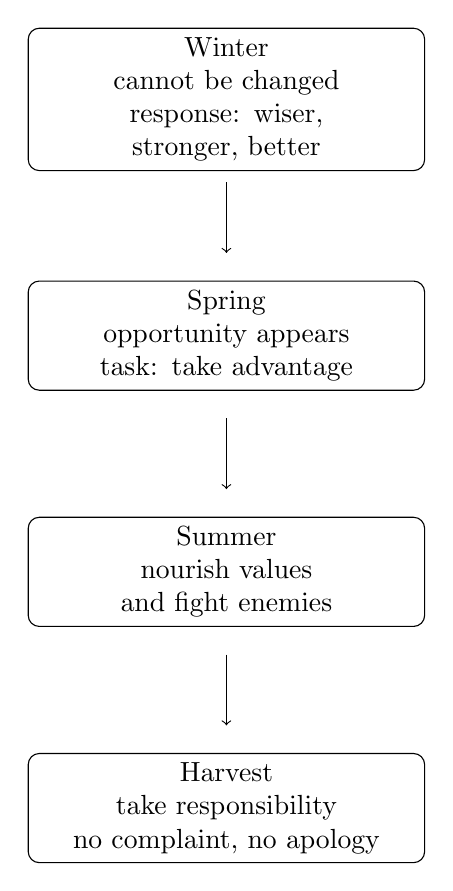
\begin{tikzpicture}[x=1cm,y=1cm]
\node[draw, rounded corners, align=center, text width=4.8cm] at (0,0) {Winter\\cannot be changed\\response: wiser, stronger, better};
\node[draw, rounded corners, align=center, text width=4.8cm] at (0,-3.0) {Spring\\opportunity appears\\task: take advantage};
\node[draw, rounded corners, align=center, text width=4.8cm] at (0,-6.0) {Summer\\nourish values\\and fight enemies};
\node[draw, rounded corners, align=center, text width=4.8cm] at (0,-9.0) {Harvest\\take responsibility\\no complaint, no apology};
\draw[->] (0,-1.05) -- (0,-1.95);
\draw[->] (0,-4.05) -- (0,-4.95);
\draw[->] (0,-7.05) -- (0,-7.95);
\end{tikzpicture}
\end{center}
\end{figure}

Winter comes first because it removes our illusion of control. We cannot change the winter:
\begin{equation}
\text{You cannot change the winter};\qquad \text{you can change yourself}.
\end{equation}
That is the subtraction on which the whole section depends. Once the season is fixed, the adjustable variable is the self. The lecture therefore answers winter with a trio:
\begin{equation}
W_3 := (\text{wiser},\ \text{stronger},\ \text{better}).
\end{equation}
This is not ornamental phrasing. It is the operational answer to adverse seasons. We go home smarter, with more ideas; we get stronger in courage, dedication, and the ability to cope; and we get better by repetition.

Here the lecture folds in Rohn's own speaking example. He stood up, did it badly, then did it again, and again, and again. The improvement rule is given almost as an iteration:
\begin{equation}
\text{do it again} \to \text{day-by-day improvement} \to \text{week-by-week improvement} \to \text{month-by-month improvement}.
\end{equation}
The moral is exact: winter is not answered by asking for another climate, but by becoming a person stronger than the climate.

Spring then enters as opportunity. Yet the lecture immediately disciplines the optimism. Spring is not self-executing:
\begin{align}
\text{spring} &\neq \text{guaranteed harvest},\\
\text{spring} &\Rightarrow \text{take advantage}.
\end{align}
The imperative is repeated in the transcript for a reason. Take advantage. Take advantage. Take advantage. This is not only advice; it is the correction of a common delusion. Nice weather does not produce a crop. We must seize the spring with our own hands.

The lecture presses the point with urgency. Spring does not last long. The farming example makes the timing concrete: one does not go bowling during planting season. Opportunity is therefore real, but time-limited. Delay is not neutral. Delay is already refusal.

\subsection{Question \& Answer}

Question: What do we do when the season is against us?

Answer: We do not spend our energy wishing for another season. The lecture's rule is to move attention from the unchangeable to the changeable. Winter asks for \(W_3\): become wiser, stronger, better. Spring asks for timely seizure. The season is acknowledged fully, but it is not allowed to become an excuse.

\section{Get Better Through the Seasons: Summer Battle and Harvest Responsibility}

Summer is where the lecture becomes both generous and combative. Growth is now possible, but growth attracts resistance. That is why summer is given a dual task:
\begin{equation}
\text{summer work} := (\text{nourish values},\ \text{fight enemies}).
\end{equation}
The lecture insists on both halves. We feed what is valuable, and we resist what would destroy it. Opportunity arrives mixed with difficulty; this is not an exception but the normal grammar of life.

The enemies are then brought inward. Some are outside us, but the most dangerous ones may be inside. The quick list is formal enough to keep as a list:
\begin{equation}
E_5 := (\text{indifference},\ \text{indecision},\ \text{doubt},\ \text{worry},\ \text{pessimism}).
\end{equation}
Each item is given an operational correction. Indifference is fought by refusing to coast too long. Indecision is fought by making decisions, even when imperfect decisions must later teach us. Doubt is fought by refusing to pick up the whole world's doubts and by refusing, above all, to doubt oneself. Worry is allowed a narrow place, but only under mastery: we are to be the master of worry, not its servant.

The business setting is preserved here through the repeated language of ``good hands.'' The audience is told to go home able to say that in its community Herbalife is in good hands. This is more than reassurance. It is the moral form of summer labor: steady hands, growing hands, intelligent hands.

Pessimism receives the lecture's sharpest formal correction:
\begin{equation}
\text{glass is half empty} \land \text{glass is half full}.
\end{equation}
The mistake of pessimism is not seeing the empty half. The mistake is treating the empty half as the whole truth. That is why Rohn says pessimism has to be educated. The correction is conjunction, not denial.

The bodily analogy that follows gives the same duality in another register:
\begin{equation}
\text{red corpuscles} \Rightarrow \text{nourish}, \qquad
\text{white corpuscles} \Rightarrow \text{fight / kill infection}.
\end{equation}
This is one of the lecture's best local models. A living body survives by giving life and by threatening back whatever would kill it. The same is true, he says, of a serious life: love and nourish, but also take sword to the enemy.

Harvest is then introduced as the final season, and the tone changes again. We are now told to own the crop:
\begin{align}
\text{harvest} &\Rightarrow \text{responsibility},\\
\text{harvest} &\Rightarrow \text{no complaint} \land \text{no apology for earned results}.
\end{align}
This is exact lecture logic. If the calls were made, the letters written, the day put together steadily, then the crop is ours and we take responsibility for it. If the job has been done well, there is no need to apologize for its returns. The lecture keeps the business particulars in view here: money is not abstracted away, but it is morally tied to lives touched and help given.

\subsection{Question \& Answer}

Question: How can we both nourish life and fight what threatens it?

Answer: By refusing the false alternative. The lecture's summer logic is explicitly two-sided. We nourish our values, our families, our customers, and our organizations; at the same time we do battle with indifference, worry, infection, threat, and anything else that would destroy those values. The corpuscle analogy is the clearest formulation: a healthy system feeds and defends at once.

\section{Absorb, Respond, Reflect, Share; Then Get Excited and Get Away}

After the long seasonal development, the lecture compresses ``get better'' into four portable verbs:
\begin{equation}
B_4 := (\text{absorb},\ \text{respond},\ \text{reflect},\ \text{share}).
\end{equation}
This is a genuine compression, not an appendix. The whole middle of the talk is being folded into habits that can travel home.

To absorb is to soak up the room, the examples, the sounds, the seriousness, the other people, and the work itself. To respond is to let life touch us rather than to walk through it armored against both pain and opportunity. To reflect is to run the tapes again, not vaguely, but at definite intervals. The lecture gives the sequence quite concretely:
\begin{align}
\text{end of day} &\to \text{go back over the day},\\
\text{end of week} &\to \text{go back over the week},\\
\text{end of month} &\to \text{go back over the month},\\
\text{end of conversation} &\to \text{go back over the conversation}.
\end{align}
This is why we may safely define
\begin{equation}
\text{reflection} := \text{gather the past and invest it in the future}.
\end{equation}
The past is not only memory; it is raw material for next year's competence.

To share is the outward turn. Here the lecture becomes almost a theory of testimony. We are not to touch people only with a marketing plan or a kit, but with life, experience, heart, and soul. Words matter because they help people see what they could not yet see. That is why the lecture says that words work miracles. Good words and testimony turn on lights.

Only after this outward movement do we arrive at the last two imperatives. First, get excited. But the lecture carefully distinguishes two kinds of excitement:
\begin{equation}
\text{deep excitement} \neq \text{surface excitement}.
\end{equation}
Noise is not the point. The desired excitement is the inward one that stirs commitment, courage, and the sentence ``Give me the chance and I will get the job done.''

Finally, get away. The lecture refuses to end in strain. Balance is demanded: family, friendship, spirituality, responsibility, work, health, money, and future must remain in live relation. Friendship is not treated sentimentally here. It is part of the causal structure of a life; nourished over years, it becomes one of the channels by which opportunity itself arrives.

\subsection{Question \& Answer}

Question: How do words and testimony become practical forces rather than empty inspiration?

Answer: In the lecture they become practical only after the earlier work has been done. First we absorb, respond, reflect, and share. First we become serious, learn, act, and get better. Then words are no longer detached slogans. They become carriers of lived experience. At that point a testimony can do something precise: it can help another person see a possibility, an opportunity, or a next step that was previously invisible.

\section{Summary}

The lecture begins with seriousness and ends with balance, but the path between them is tightly staged. Seriousness first raises the stakes of life. The \$400 million arithmetic then gives seriousness a measurable object. Education corrects the fantasy that excitement is enough. Philosophy explains why common winds still produce unequal destinations. Action enters as the cleansing of neglect. The seasons then organize growth across time: winter asks for self-strengthening, spring for timely seizure, summer for nourishment and battle, harvest for responsibility. Finally, the whole structure is compressed into absorb, respond, reflect, share, deep excitement, and balanced living.

What looks at first like a string of aphorisms is therefore a real program. In the lecture's own order, it remains
\begin{equation}
G_6 := (\text{get serious},\ \text{get smart},\ \text{get going},\ \text{get better},\ \text{get excited},\ \text{get away}),
\end{equation}
and the chapter is faithful only if we let each term arise when the previous one has shown its limit.